\documentclass[12pt]{article}

% URLs and hyperlinks ---------------------------------------
\usepackage{hyperref}
\hypersetup{
	colorlinks=true,
	linkcolor=blue,
	filecolor=magenta,      
	urlcolor=blue,
}
\usepackage{xurl}
%---------------------------------------------------

\usepackage{float}
\usepackage{adjustbox}
\usepackage{graphicx}
\usepackage{rotating}
\usepackage{mathtools}
\usepackage{enumitem}
\usepackage{gensymb}

\usepackage{xepersian}
\settextfont{Yas}

\title{گزایش کار آزمایش هشتم}
\author{	گروه: \\	اریسا احسانی \\	سید حسین حسینی \\	مهدی حق‌وردی \\ \\	شعبه شش
}
\date{}
\renewcommand{\arraystretch}{1.4}

\begin{document}
\maketitle
\newpage

\begin{figure}[H]
\begin{center}
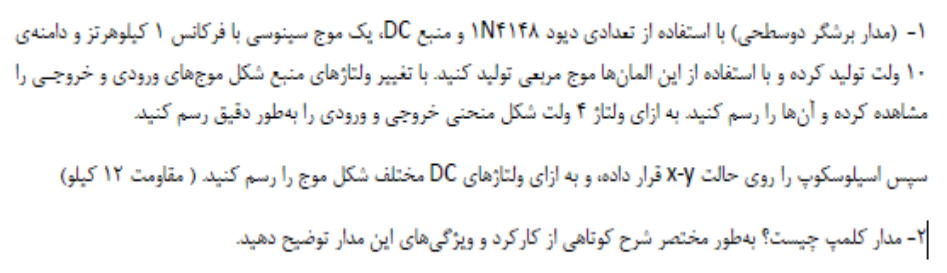
\includegraphics[width=\textwidth, height=5cm]{./images/8.1}
\end{center}
\end{figure}

\begin{figure}[H]
	\begin{flushleft}
		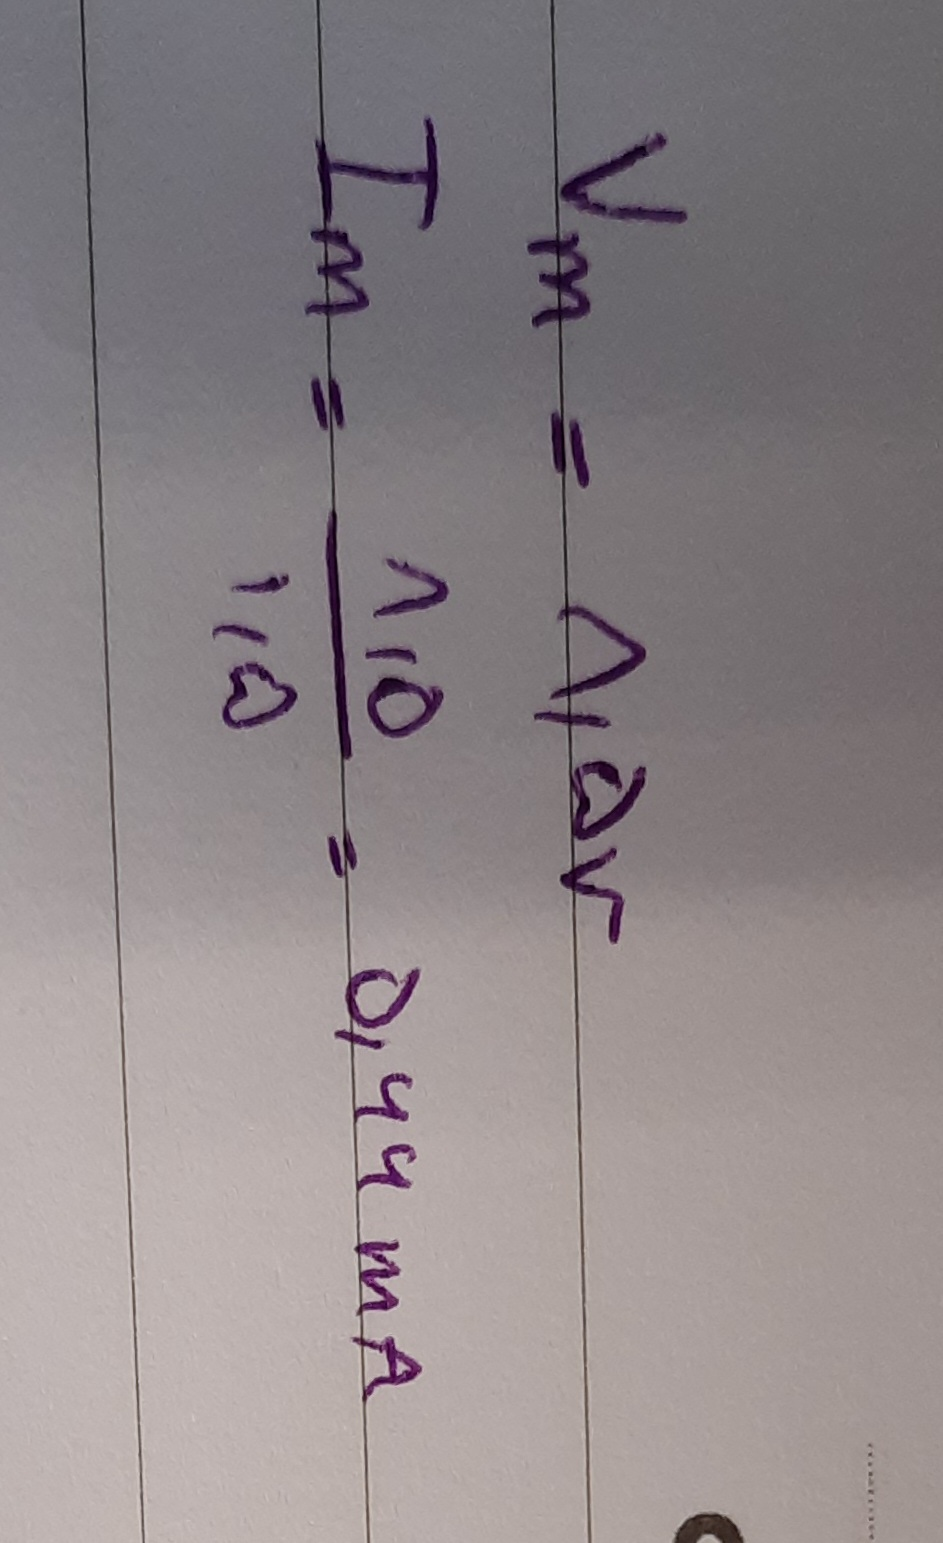
\includegraphics[width=5cm, height=5cm, angle=90]{./images/8.i.1}
	\end{flushleft}
\end{figure}

\begin{figure}[H]
	\begin{flushleft}
		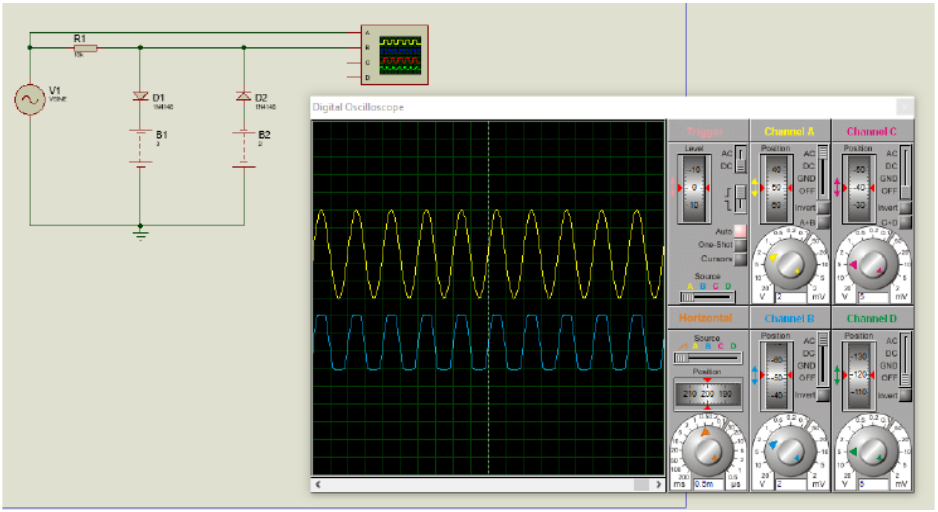
\includegraphics[width=0.8\textwidth, height=6cm]{./images/8.2}
	\end{flushleft}
\end{figure}

به ازای ۴ ولت شکل منحنی ورودی و خروجی 
\begin{figure}[H]
	\begin{center}
		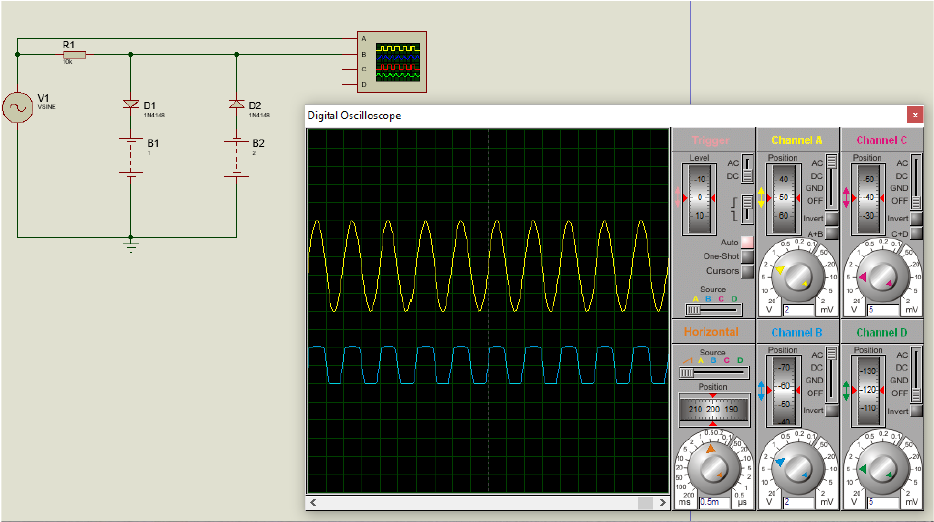
\includegraphics[width=\textwidth, height=8cm]{./images/8.3}
	\end{center}
\end{figure}
\begin{figure}[H]
	\begin{center}
		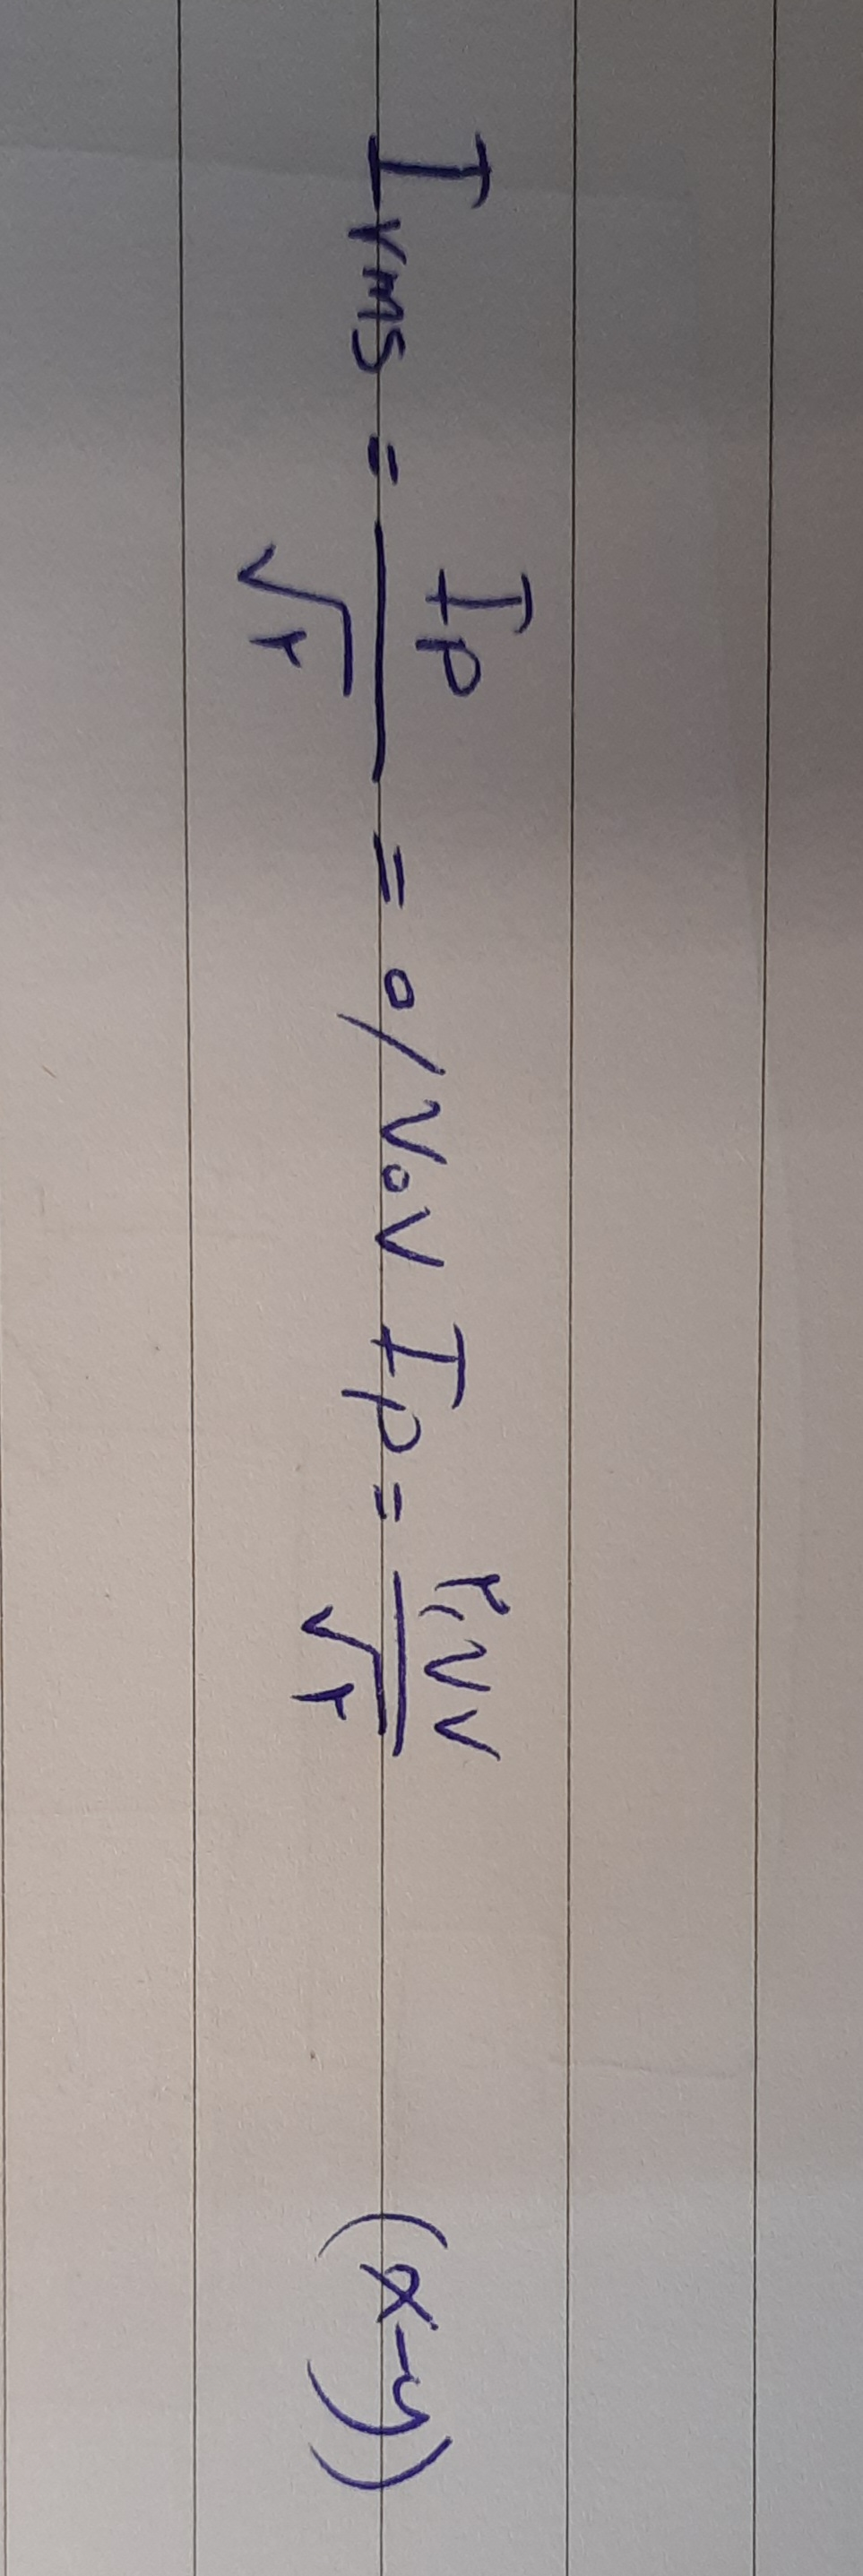
\includegraphics[width=7cm, height=\textwidth, angle=90]{./images/8.i.2}
	\end{center}
\end{figure}
\begin{figure}[H]
	\begin{center}
		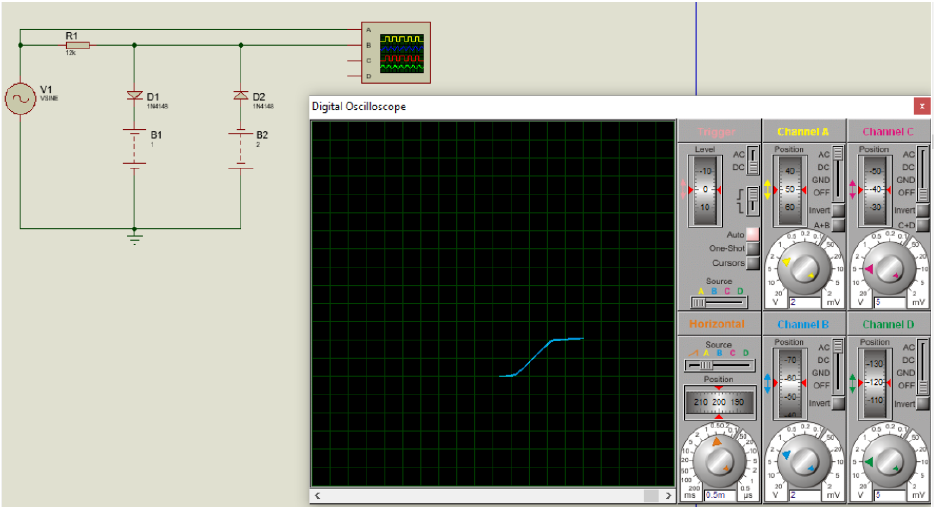
\includegraphics[width=\textwidth, height=8cm]{./images/8.4}
	\end{center}
\end{figure}

پاسخ سوال ۲:
مدارات برش دیودی به منظور برش دادن قسمت مثبت یا منفی از یک شکل موج متناوب مورد استفاده قرار می‌گیرند. اما یک مدار کلمپ دیودی را می‌توان یک مدار شیفت دهنده سطح در نظر گرفت. این مدار با استفاده از مقاومت، خازن و دیود به صورت عملی پیاده‌سازی می‌شود.

تفاوت اصلی بین یک مدار کلیپر یا برش دیودی و مدار کلمپ در این است که مدار برش شکل موج سیگنال ورودی را تغییر می‌دهد، در حالی که مدار کلمپ فقط سطح \lr{DD} سینگال را دستخوش تغییر می‌کند. لازم به ذکر است که سطح ولتاژ \lr{DC} در یک سینگال برابر با مقدار متوسط آن سیگنال در نظر گرفته می‌شود.
۳. مدار کلمپ را رسم کنید. ولتاژ \lr{DC} را کم و زیاد کرده و خروجی را بدست آوردید.
\begin{figure}[H]
	\begin{center}
		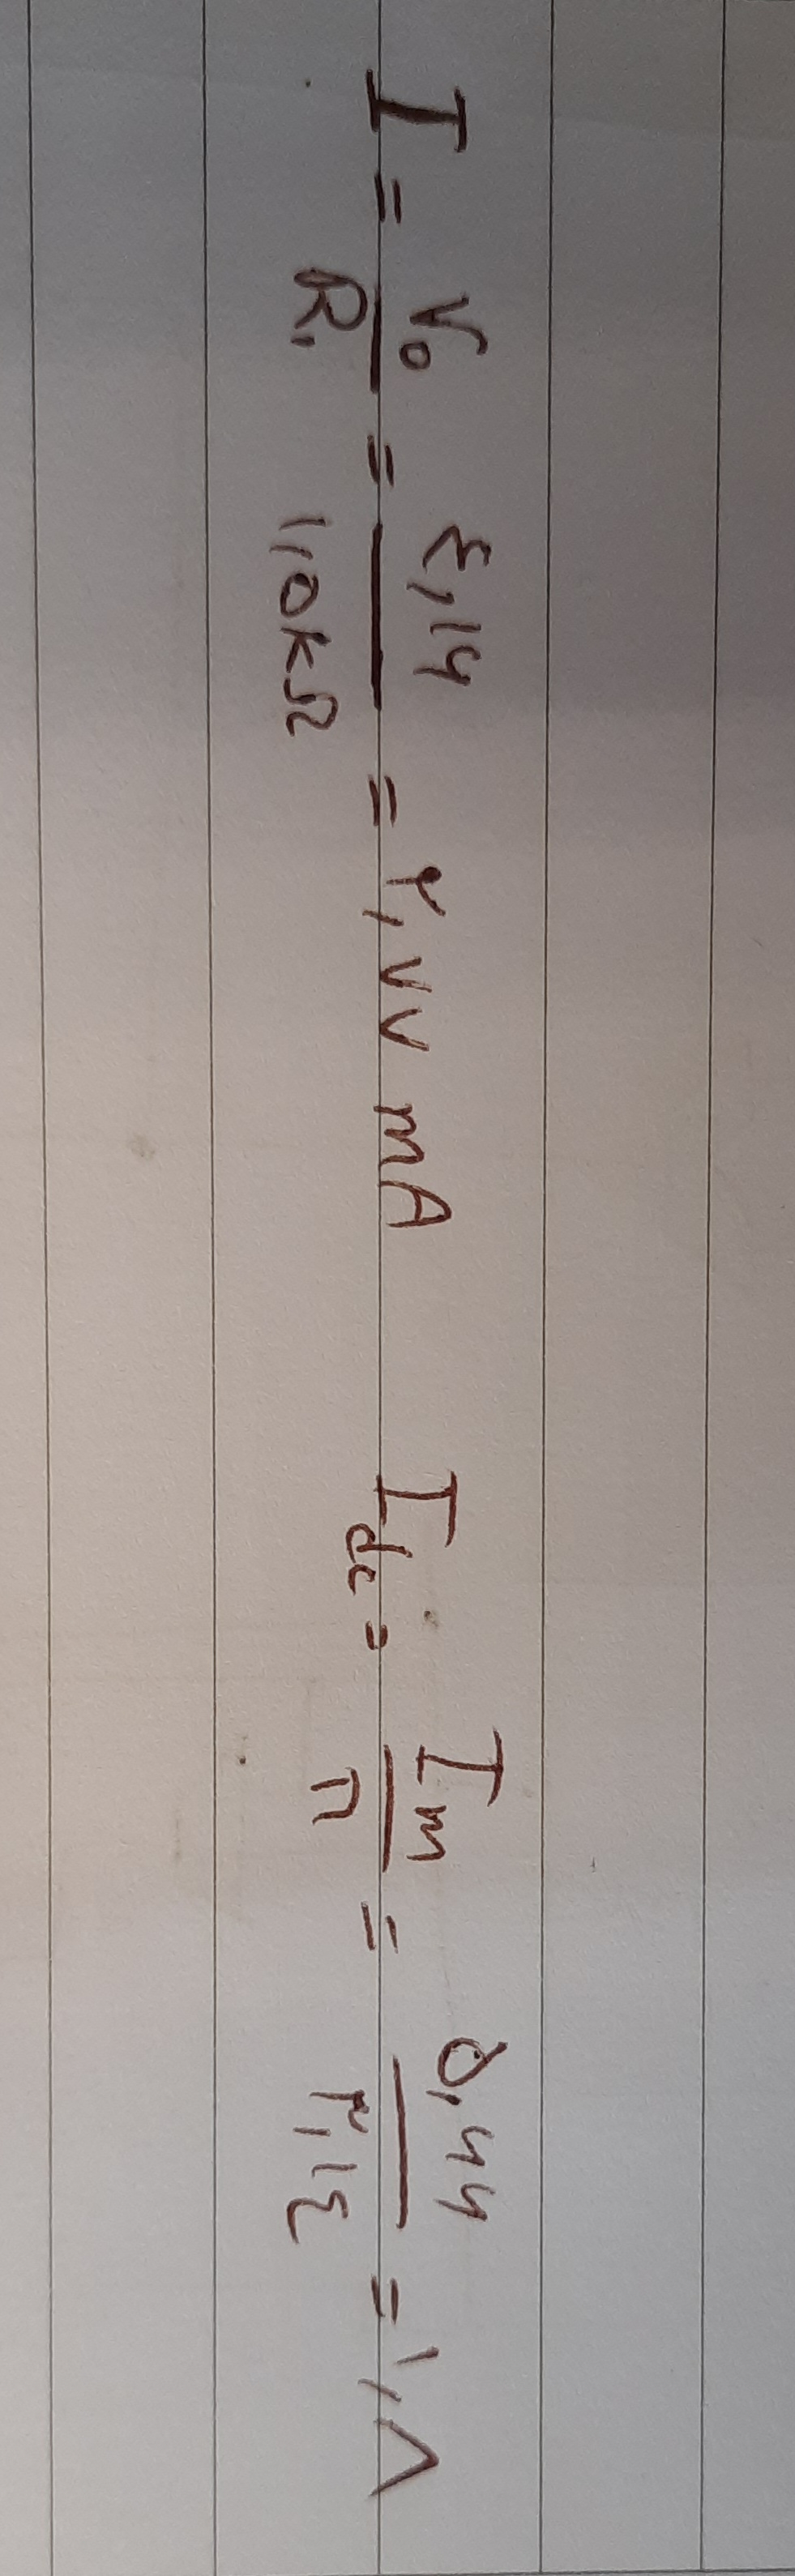
\includegraphics[width=6cm, height=\textwidth, angle=90]{./images/8.i.3}
	\end{center}
\end{figure}

\begin{figure}[H]
	\begin{center}
		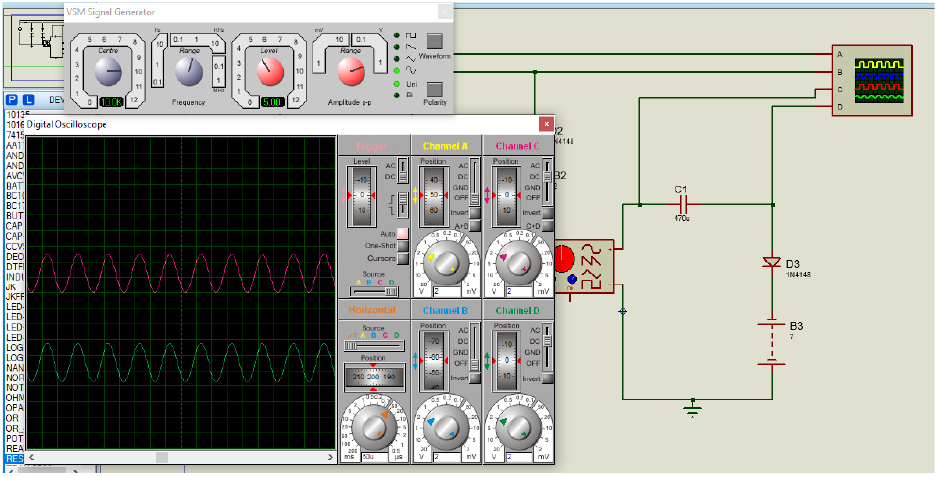
\includegraphics[width=\textwidth, height=8cm]{./images/8.5}
	\end{center}
\end{figure}
\begin{figure}[H]
	\begin{center}
		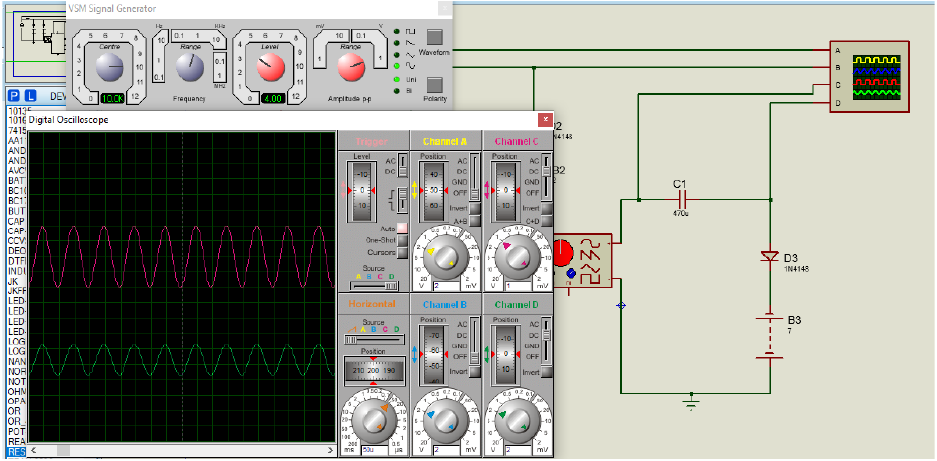
\includegraphics[width=\textwidth, height=8cm]{./images/8.6}
	\end{center}
\end{figure}

کلمپ منفی است چون بایاس منفی متصل شده است. در طول نیم سیکل مثبت از سیگنال ورودی به مدار، دیود توسط هر دو ولتاژ تغذیه‌ی ورودی و نیز ولتاژ باتری در مود بایاس مستقیم قرار می‌گیرد. در نتیجه، جریان در خازن جاری می‌شود و آن را شارژ می‌کند. در طول نیم سیکل منفی از سیگنال ورودی، زمانی که ولتاژ تغذیه مدار از ولتاژ باتری کمتر باشد، ولتاژ باتری دیود را در مود بایاس مستقیم قرار می‌دهد و زمانی که ولتاژ ورودی تغذیه از ولتاژ باتری بزرگ‌تر شود، دیود توسط ولتاژ تغذیه‌ ورودی در مود بایاس معکوس قرار می‌گیرد و در نتیجه دلیل دلیل سیگنال در خروجی ظاهر می‌شود. با افزایش ویتاژ‌ \lr{DC} خروجی به سمت منفی پرش بیشتری می‌کند.

۴. مدار یک‌سوساز نیم موج را رسم کرده، از ترانسفوماتور ۲۲۰ ولت به ۹ ولت استفاده کنید

\begin{figure}[H]
	\begin{center}
		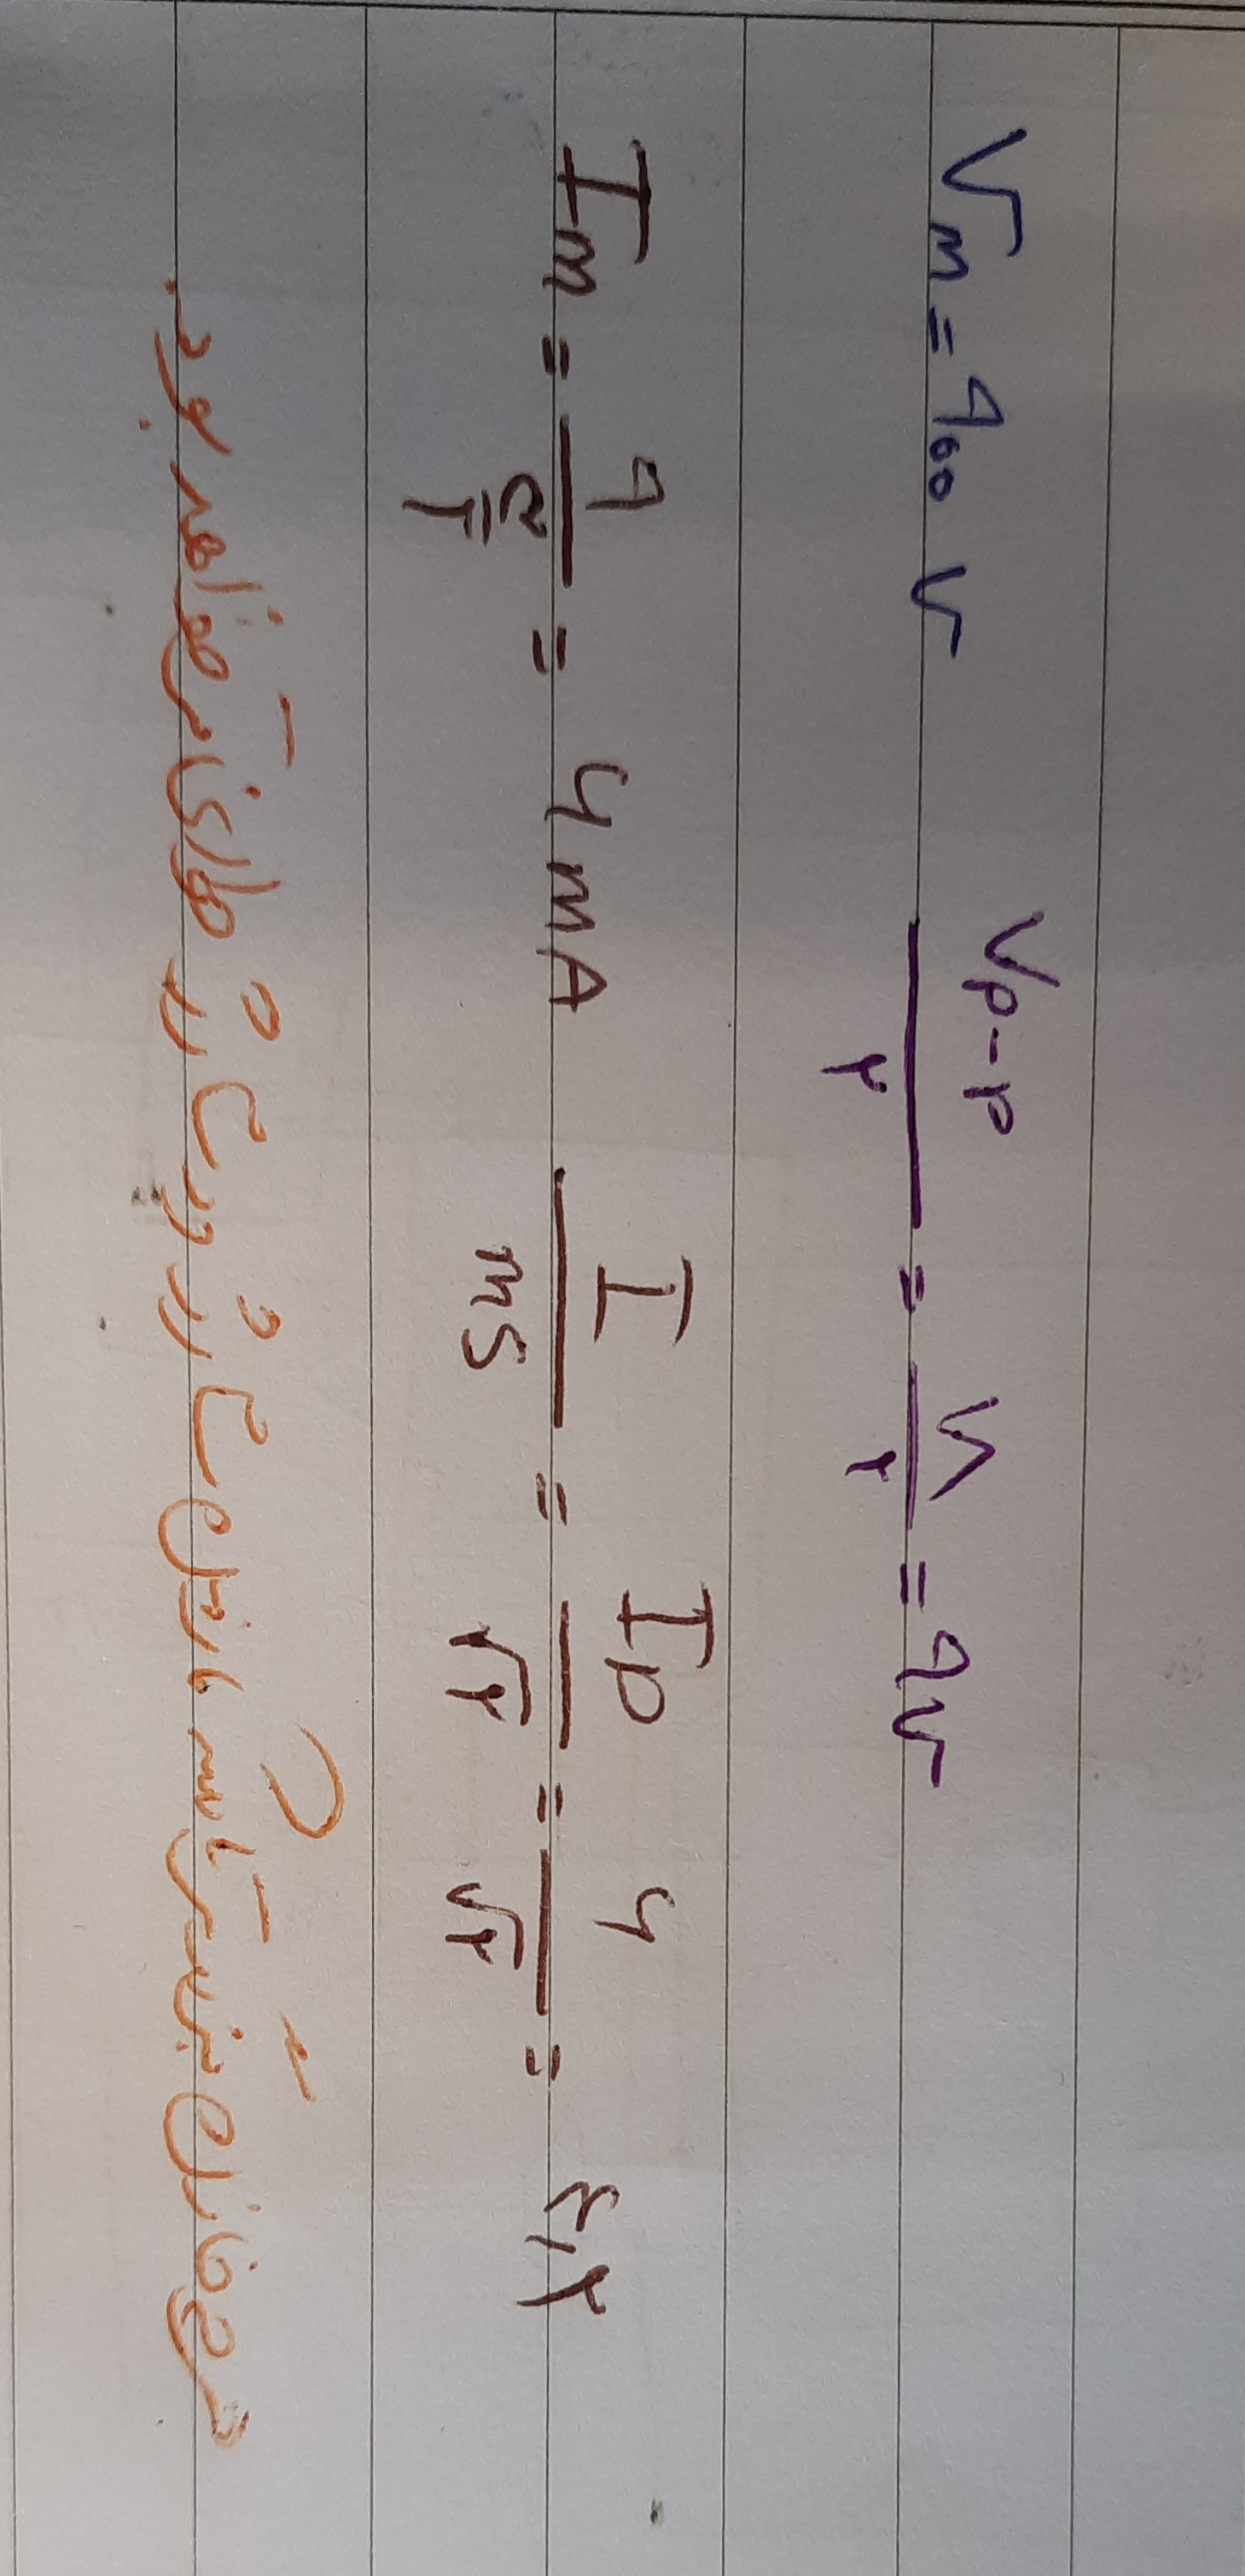
\includegraphics[width=8cm, height=\textwidth, angle=90]{./images/8.i.4}
	\end{center}
\end{figure}

\begin{figure}[H]
	\begin{center}
		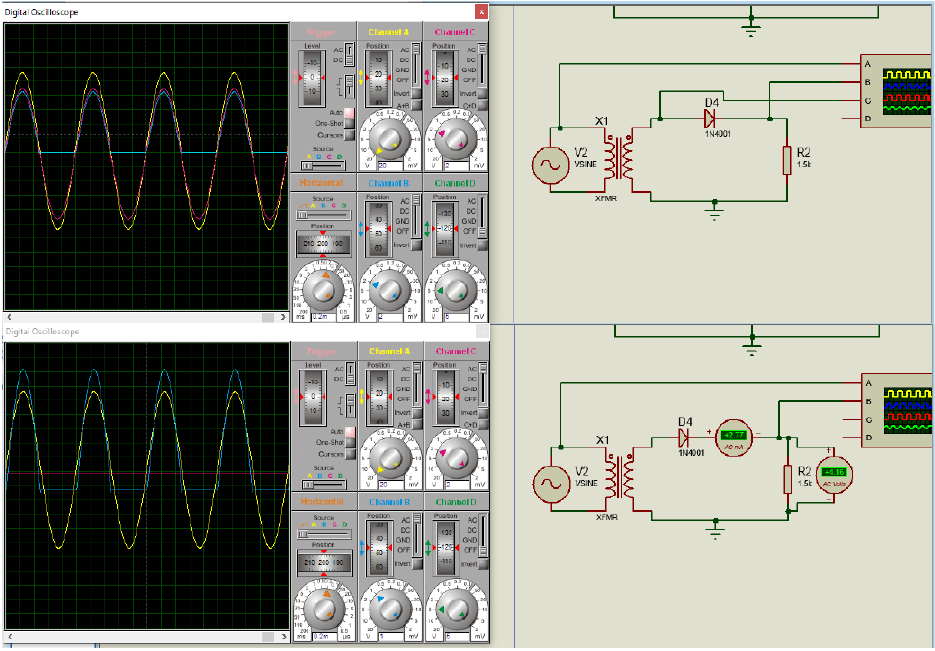
\includegraphics[width=\textwidth, height=8cm]{./images/8.7}
	\end{center}
\end{figure}

۵. یکسوساز تمام‌ موج با بار $2.2$ کیلو و خروجی ترانس ۱۲ ولت
\begin{figure}[H]
	\begin{center}
		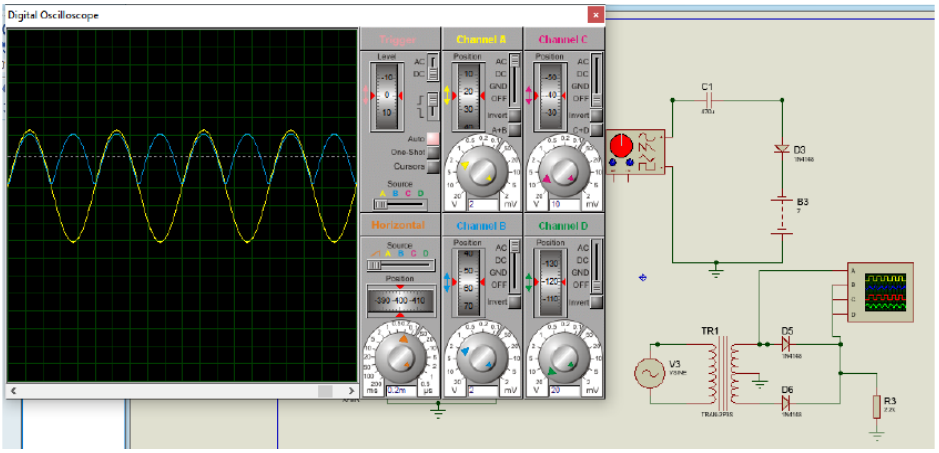
\includegraphics[width=\textwidth, height=8cm]{./images/8.8}
	\end{center}
\end{figure}

۶. پاسخ سوال شش
\begin{figure}[H]
	\begin{center}
		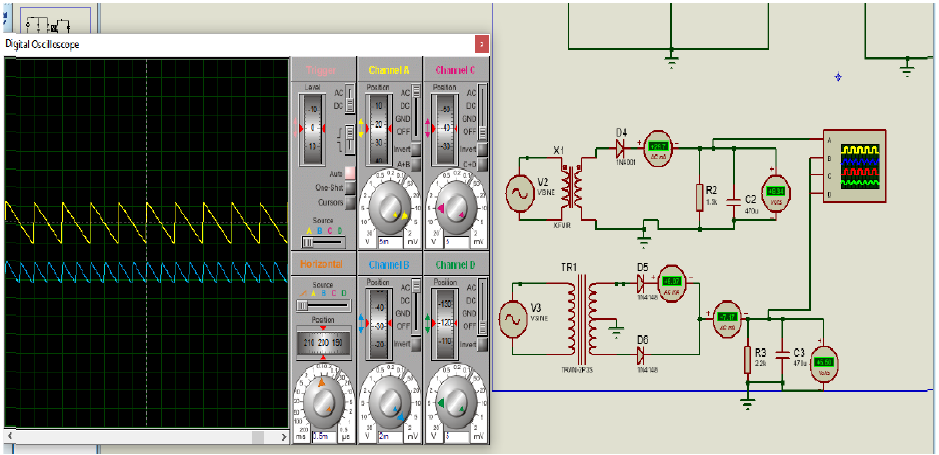
\includegraphics[width=\textwidth, height=8cm]{./images/8.9}
	\end{center}
\end{figure}
\begin{figure}[H]
	\begin{center}
		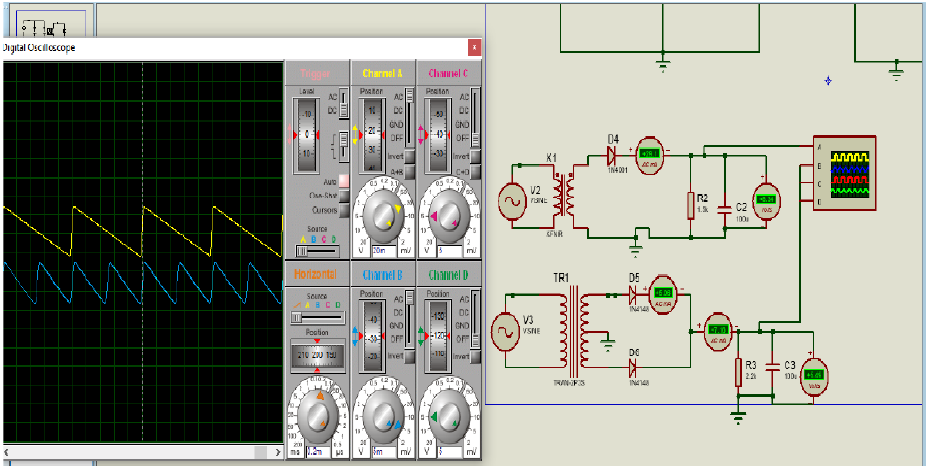
\includegraphics[width=\textwidth, height=8cm]{./images/8.10}
	\end{center}
\end{figure}

۷. پاسخ سوال هفت
\begin{figure}[H]
	\begin{center}
		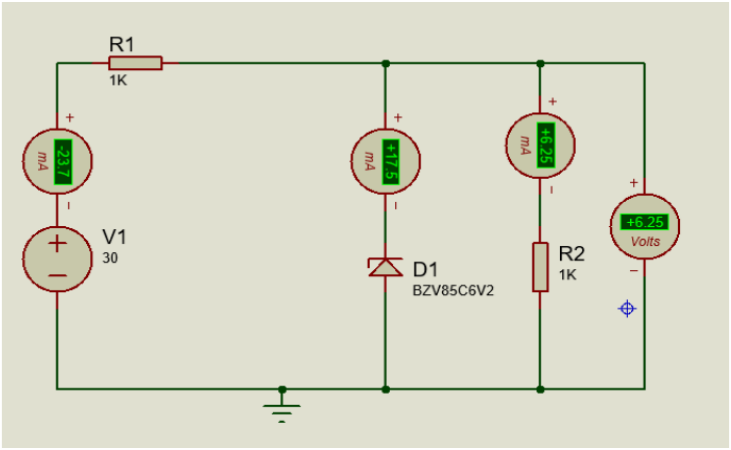
\includegraphics[width=\textwidth, height=8cm]{./images/8.11}
	\end{center}
\end{figure}

\begin{latin}
\begin{table}[H]
\begin{adjustbox}{width=\textwidth}
\begin{tabular}{|c|c|c|c|c|c|c|c|c|}
\hline
$V_i$ & 9 & 12 & 15 & 18 & 21 & 25 & 27 & 30 \\
\hline
\hline
$V_O$ & 4.5 & 6 & 6.20 & 6.22 & 6.23 & 6.24 & 6.25 & 6.25 \\
\hline
$I_S$ & 4.5 & 6 & 8.8 & 11.8 & 14.9 & 18.8 & 20.8 & 23.7 \\
\hline
$I_L$ & 4.5 & 6 & 6.2 & 6.22 & 6.23 & 6.24 & 6.25 & 6.25 \\
\hline
$I_z$ & 0 & 0 & 2.6 & 5.56 & 8.54 & 12.5 & 14.5 & 17.5 \\
\hline
\end{tabular}
\end{adjustbox}
\end{table}
\end{latin}


\begin{figure}[H]
	\begin{center}
		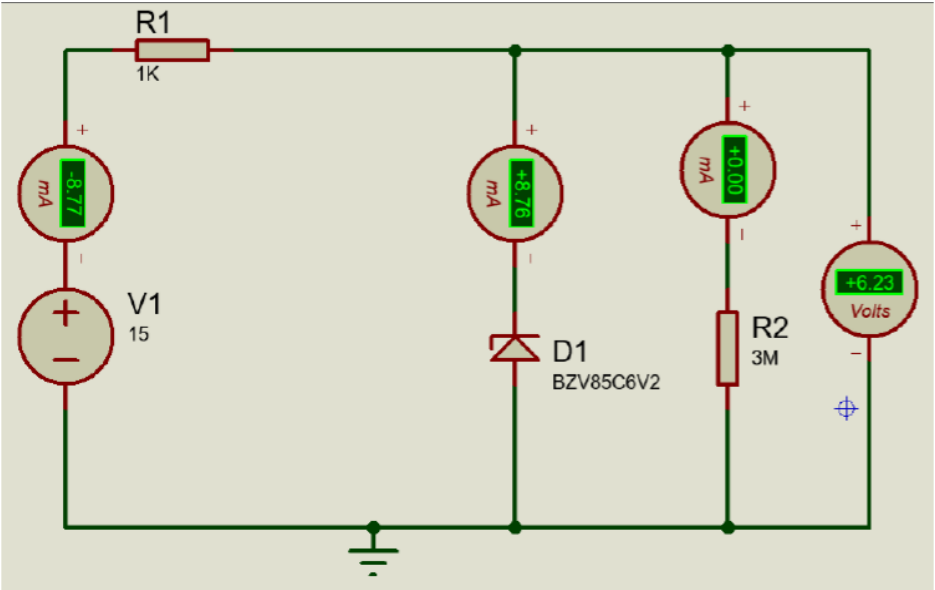
\includegraphics[width=\textwidth, height=8cm]{./images/8.12}
	\end{center}
\end{figure}


\begin{latin}
\begin{table}[H]
\begin{adjustbox}{width=\textwidth}
\begin{tabular}{|c|c|c|c|c|c|c|}
\hline
$R_1$ & 0.33 & 0.56 & 1 & 1.5 & 2.2 & $\infty$ \\
\hline
\hline
$V_O$ & 3.72 & 5.38 & 6.2 & 6.21 & 6.22 & 6.23 \\
\hline
$I_S$ & 11.3 & 9.62 & 8.8 & 8.79 & 8.75 & 8.77 \\
\hline
$I_I$ & 11.3 & 9.62 & 6.2 & 4.14 & 2.83 & 0 \\
\hline
$I_Z$ & 0 & 0 & 2.6 & 6.46 & 5.95 & 8.76 \\
\hline
\end{tabular}
\end{adjustbox}
\end{table}
\end{latin}
\end{document}